\documentclass[a4paper]{article}
\def\DOCTITLE{CSC3423 Biocomputing}
% Set document attributes
\title{\DOCTITLE}

\usepackage{fullpage}
\usepackage{scrextend}
\usepackage{titlesec}
\usepackage{fancyhdr}
\usepackage{amsmath}
\usepackage{amssymb}

% Handle graphics correctly
\ifx\pdftexversion\undefined
\usepackage{graphicx}
% \usepackage[dvips]{graphicx}
\else
\usepackage[pdftex]{graphicx}
\DeclareGraphicsRule{*}{mps}{*}{}
\fi

% Setup headers and footers
\pagestyle{fancy}
\lhead{}
\chead{\DOCTITLE}
\rhead{}
\rfoot{}
\cfoot{\thepage}
\lfoot{}

% New page for each section
% \newcommand{\sectionbreak}{\clearpage}

% Set header and footer sizes
\renewcommand{\headrulewidth}{0.4pt}
\renewcommand{\footrulewidth}{0.4pt}
\setlength{\headheight}{15.2pt}
\setlength{\headsep}{15.2pt}

\setlength{\parskip}{5pt plus 1pt minus 1pt}
\setlength{\parindent}{0pt}

\newcommand{\Forall}{\;\forall\;}
\newcommand{\Mod}{\: mod \:}


\begin{document}

\tableofcontents

\section{Overview}
\label{sec:overview}

\begin{table}[h]
  \centering
  \begin{tabular}{@{}l|cccccc@{}}
    \toprule
    Problem Type     & GA/GP/MA     & NN          & ACO           & PSO         & CA          & MC          \\
    \midrule
    Optimisation     & \checkmark   &             & (\checkmark)  & \checkmark  &             &             \\
    Machine Learning & \checkmark   & \checkmark  & (\checkmark)  & \checkmark  &             &             \\
    Control          & \checkmark   & \checkmark  & (\checkmark)  & \checkmark  &             &             \\
    Simulation       & (\checkmark) &             &               &             & \checkmark  & \checkmark  \\
    \bottomrule
  \end{tabular}
  \caption{Suitability of algorithms to problems}
  \label{tab:suitability}
\end{table}

\begin{description}
  \item[GA]   Genetic Algorithm
  \item[GP]   Genetic Programming
  \item[MA]   Memetic Algorithm
  \item[NN]   Neural Network
  \item[ACO]  Ant Colony Optimisation
  \item[PSO]  Particle Swarm Optimisation
  \item[CA]   Cellular Automata
  \item[MC]   Membrane Computing
\end{description}

\section{Genetic Algorithms}
\label{sec:ga}

\subsection{Biological Inspiration}

\Para{Natural selection}

Principle that every slight change in a trait that is beneficial is preserved.

Individuals that have traits that allow them to be better adapted to the
environment are more likely to reproduce, traits are then passed to later
generations.

\Para{Genetics}

Candidate solutions to a problem represented in a chromosome composed of several
genes.

Genes are passed from generation to generation with small changes (mutations).

\subsection{Overview}

\begin{figure}[h!]
  \centering
  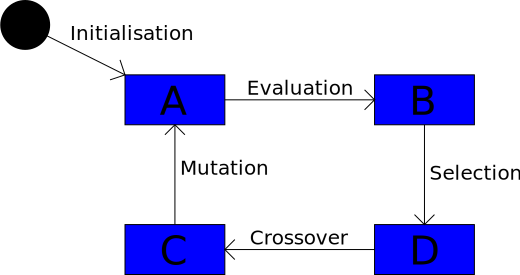
\includegraphics[width=0.5\textwidth]{out/ga_workflow.eps}
  \caption{Genetic Algorithm Workflow}
  \label{fig:ga_workflow}
\end{figure}
\FloatBarrier

\Para{Pseudocode}

\begin{listing}[h]
  \begin{minted}{python}
    population = init_random_population()
    iteration = 0
    while iteration < num_interations:
      evaluate(population)
      population = selection(population)
      population = crossover(population)
      population = mutation(population)
      iteration++
    best = get_best_individual(population)
    return best
  \end{minted}
  \caption{Genetic algorithm pseudocode}
  \label{listing:ga_pseudocode}
\end{listing}

\subsection{Population}

\begin{itemize}
  \item Set of possible solutions to the problem
  \item Most often a set (chromosome) of variables (genes)
  \item Initial population created at random
\end{itemize}

\subsection{Evaluation}

\begin{itemize}
  \item Giving a "goodness" value to each candidate solution
  \item Uses a fitness function which takes a candidate solution and determines
        how well it solves the problem
\end{itemize}

\subsection{Selection}

\begin{itemize}
  \item Choosing individuals to be in the next population
  \item Rewards best individuals (i.e. those with the best fitness values)
\end{itemize}

\subsubsection{Roulette Wheel Selection}

\begin{itemize}
  \item Probability of selection is proportional to fitness of individual
  \item Make as many selections (spins of wheel) as individuals to be selected
  \item Individuals may be selected multiple times
\end{itemize}

\begin{figure}[h!]
  \centering
  \includegraphics[width=0.4\textwidth]{out/roulette_wheel_selection.eps}
  \caption{Roulette Wheel Selection}
  \label{fig:roulette_wheel_selection}
\end{figure}
\FloatBarrier

\subsubsection{Stochastic Universal Sampling}

\begin{itemize}
  \item Similar to Roulette Wheel Selection
  \item Do one spin but divide "pointer" into as many individuals to be selected
\end{itemize}

\begin{figure}[h!]
  \centering
  \includegraphics[width=0.4\textwidth]{out/stochastic_universal_sampling.eps}
  \caption{Stochastic Universal Sampling}
  \label{fig:stochastic_universal_sampling}
\end{figure}
\FloatBarrier

\subsubsection{Tournament Selection}

\begin{itemize}
  \item Select the best individual from a randomly selected subset of the
        population
\end{itemize}

\begin{listing}[h]
  \begin{minted}{python}
    new_population = []
    while population.size() > 0:
      tournament = select_random_subset(population, tournament_size)
      tournament = sort_by_fitness(tournament)
      new_population.add(tournament[0])
    return new_population
  \end{minted}
  \caption{Tournament selection pseudocode}
  \label{listing:ga_tournament_selection_pseudocode}
\end{listing}

\subsubsection{Truncation Selection}

\begin{itemize}
  \item Keep only the best $n$ individuals in a population
\end{itemize}

\subsubsection{Comparison of selection methods}

\begin{description}
  \item[Roulette Wheel \& Stochastic Selection] \hfill \\
    \begin{itemize}
      \item Fitness proportionate
      \item Chance of being selected is proportionate to fitness value
      \item Selection becomes random when fitness values are close (e.g. in
            later GA iterations)
    \end{itemize}

  \item[Tournament \& Truncation Selection] \hfill \\
    \begin{itemize}
      \item Rank based
      \item Best individual will always win a tournament
      \item More stable selection pressure
    \end{itemize}

\end{description}

\subsection{Crossover}

\begin{itemize}
  \item Exchanging genes between two individuals
  \item Takes two individuals from the population and generates two offspring
  \item e.g. For a bit array, one offspring takes first section of array and
        second of another, and vice-versa
  \item e.g. For numerical genes the blend alpha operator picks a random value
        between the two parent genes
\end{itemize}

\subsection{Mutation}

\begin{itemize}
  \item Making small/subtle modifications to an individual
  \item Probability $P_{m}$ of mutation can be set either per chromosome or per
        individual
  \item e.g. Randomly flipping a bit where the chromosome is a bit array
  \item e.g. Adding a random value to a numerical gene
\end{itemize}

\subsection{Replacement}

\begin{itemize}
  \item Alternative to generational genetic algorithm
  \item Steady state genetic algorithm
    \begin{itemize}
      \item Elitism
      \item Selection chooses two parents who produce two offspring
      \item Offspring are inserted into the parent population, replacing the
            two individuals with lowest fitness
    \end{itemize}
\end{itemize}

\subsection{Knowledge Representation}

Nominal attributes:

\begin{itemize}
  \item Set of rules and logic predicates
\end{itemize}

Real valued attributes:

\begin{itemize}
  \item Hyperrectangle ($n$ dimension rectangle)
  \item Hyperellipsoid ($n$ dimension circle)
  \item Decision trees
  \item Synthetic prototypes (e.g. nearest neighbour)
  \item Linear classifier (separate instances of classes for classification
        problems)
\end{itemize}

\begin{figure}[h]
  \centering
  \begin{subfigure}[b]{0.4\textwidth}
    \includegraphics[width=\textwidth]{out/kr_decision_tree.eps}
    \caption{Decision Tree}
  \end{subfigure}
  \begin{subfigure}[b]{0.4\textwidth}
    \includegraphics[width=\textwidth]{out/kr_nearest_neighbour.eps}
    \caption{Nearest Neighbour}
  \end{subfigure}
  \caption{}
  \label{fig:ga_knowledge_representations}
\end{figure}
\FloatBarrier

\subsection{Tuning}

\begin{itemize}
  \item Required to ensure a proper evolutionary process
  \item GA learns well when exploration and exploitation are balanced
    \begin{description}
      \item[Exploration]
        Directing population to unknown areas of the problem space
      \item[Exploitation]
        Directing the population to most promising (based on fitness) parts of
        the problem space
    \end{description}
  \item Too much exploitation can lead to convergence to a sub-optimal solution
        (premature convergence)
    \begin{itemize}
      \item If population is too similar then crossover operator no longer
            provides effective exploration
    \end{itemize}
  \item Too much exploration risks:
    \begin{itemize}
      \item Slowing down the learning process
      \item If probabilities are too high then crossover and mutation may harm
            the overall population fitness
    \end{itemize}
  \item Innovation time $t_{i}$ is the average time taken to create an
        individual with better fitness than the current best individual
\end{itemize}

\subsection{Machine Learning}

\begin{description}
  \item[Supevised learning] \hfill \\
    \begin{itemize}
      \item Learning to solve a problem
      \item If output is discrete \RArrow Classification (output value known as
            a class)
      \item If output is continuous \RArrow Regression
      \item Use a training set to train the genetic algorithm and a testing set
            to verify the generated model
      \item Optimise initialisation by creating initial population based on
            training data
    \end{itemize}

  \item[Unsupervised learning] \hfill \\
    \begin{itemize}
      \item Identifying patters/clusters
    \end{itemize}

\end{description}

\subsection{Parallel Genetic Algorithms}

\begin{itemize}
  \item Genetic algorithms tend to be slow
  \item Majority of genetic operations can be parallelised (all but crossover)
  \item Several systems exist for this:
    \begin{description}
      \item[Master-Slave model]
        GA cycle is is run on master, slaves perform operations
      \item[Island Model]
        Population is divided across nodes
      \item[Cellular GA]
        Population distributed across 2D lattice
    \end{description}
\end{itemize}

\section{Genetic Programming}
\label{sec:gp}

\begin{itemize}
  \item Very similar concept to Genetic Algorithms \ref{sec:ga}
  \item Instead of evolving a solution, evolve a program

\end{itemize}

\subsection{Program Representation}

\begin{itemize}
  \item Classic method is to represent programs as a tree representing a
        formula
  \item Modern methods can also create other representations
    \begin{itemize}
      \item e.g. Cartesian Genetic Programming creates graphs
    \end{itemize}
  \item Internal nodes of tree are functions/operations
  \item Leaves are either variables/parameters or constants
    \begin{itemize}
      \item Constants can be predefined or assigned a random value within a
            predefined range
    \end{itemize}
\end{itemize}

\Para{Example}

Figure \ref{fig:gp_tree_example} shows a tree representing the equation:
\[
  \frac{4 + P3}{P1 - sin(P2)}
\]

\begin{figure}[h!]
  \centering
  \includegraphics[width=0.3\textwidth]{out/gp_tree_example.eps}
  \caption{Example Tree}
  \label{fig:gp_tree_example}
\end{figure}
\FloatBarrier

\subsection{Initialisation}

\begin{itemize}
  \item Initial tree is generated randomly
  \item Maximum depth of tree is predefined
  \item Strategies for generation:
    \begin{description}
      \item[Grow] \hfill \\
        Generate a tree at random with leaves up to the maximum depth
      \item[Fill] \hfill \\
        Generate a tree at random with all leaves at the maximum depth
      \item[Hybrid] \hfill \\
        For each level of depth, initialise a uniform number of trees, half of
        which using Grow and half using Full
    \end{description}
\end{itemize}

\begin{figure}[h]
  \centering
  \begin{subfigure}[t!]{0.4\textwidth}
    \includegraphics[width=0.5\textwidth]{out/gp_tree_grow.eps}
    \caption{Grow}
  \end{subfigure}
  \begin{subfigure}[t!]{0.4\textwidth}
    \includegraphics[width=0.8\textwidth]{out/gp_tree_fill.eps}
    \caption{Fill}
  \end{subfigure}
  \caption{Tree initialisation}
  \label{fig:gp_initialisation}
\end{figure}
\FloatBarrier

\subsection{Evaluation/Execution}

\begin{itemize}
  \item Evaluation is done by averaging error over all test cases, giving a
        fitness value
  \item Recursive execution is easy but inefficient
  \item Converting a tree to Reverse Polish Notation solves problem
\end{itemize}

\begin{listing}[h]
  \begin{minted}{text}
    for each element e:
      if e is value:
        push e to the stack
      else if e is operator:
        pop as many elements from the stack as the operator has parameters
        execute the operator
        push the result to the stack
    return value at top of stack
  \end{minted}
  \caption{Genetic programming execution pseudocode}
  \label{listing:gp_eval_pseudocode}
\end{listing}

\subsection{Crossover}

Exchange subtrees between parents.

\Para{Example}

\begin{figure}[h]
  \centering
  \begin{subfigure}[t!]{0.4\textwidth}
    \includegraphics[width=0.8\textwidth]{out/gp_tree_example.eps}
  \end{subfigure}
  \begin{subfigure}[t!]{0.4\textwidth}
    \includegraphics[width=0.8\textwidth]{out/gp_tree_example_mutation.eps}
  \end{subfigure}
  \caption{Tree crossover parents}
  \label{fig:gp_crossover_parents}
\end{figure}
\FloatBarrier

\begin{figure}[h]
  \centering
  \begin{subfigure}[t!]{0.4\textwidth}
    \includegraphics[width=0.8\textwidth]{out/gp_tree_child_1.eps}
  \end{subfigure}
  \begin{subfigure}[t!]{0.4\textwidth}
    \includegraphics[width=0.8\textwidth]{out/gp_tree_child_2.eps}
  \end{subfigure}
  \caption{Tree crossover children}
  \label{fig:gp_crossover_children}
\end{figure}
\FloatBarrier

\subsection{Mutation}

Replace entire subtrees with a randomly generated subtree.

\Para{Example}

\begin{figure}[h]
  \centering
  \begin{subfigure}[t!]{0.4\textwidth}
    \includegraphics[width=0.8\textwidth]{out/gp_tree_example.eps}
    \caption{Before}
  \end{subfigure}
  \begin{subfigure}[t!]{0.4\textwidth}
    \includegraphics[width=0.8\textwidth]{out/gp_tree_example_mutation.eps}
    \caption{After}
  \end{subfigure}
  \caption{Tree mutation}
  \label{fig:gp_mutation}
\end{figure}
\FloatBarrier

\subsection{Bloat}

\begin{itemize}
  \item Growth of program tree without improvement in fitness
  \item Bloat can affect any evolutionary paradigm where the representation
        has variable length
  \item Solutions:
    \begin{description}
      \item[Restrict tree depth] \hfill \\
        May affect evolutionary process making it unable to find a good
        solution
      \item[Simplification] \hfill \\
        Very difficult to do efficiently
      \item[Add fitness penalty to large trees] \hfill \\
        Smaller fitness for solutions with larger trees
      \item[Consider tree size in selection] \hfill \\
        When two individuals have equal fitness, prefer the smaller tree
    \end{description}
\end{itemize}

\subsection{Applications}

\begin{description}
  \item[Regression] \hfill \\
    Reverse engineering a mathematical formula given a dataset of output values
    for given input values.

    This gives an approximation of the original formula that created the
    dataset.

  \item[Generating Electronic Circuits] \hfill \\
    Tree topology defines schematic.

    Leaves define component values (inductance, capacitance, etc.).

  \item[Control] \hfill \\
    Optimising gains of a PID controller.

  \item[Puzzle Solvers] \hfill \\
    e.g. FreeCell solver using hybrid genetic algorithm and genetic
    programming.

  \item[Generation of Audio Synhesizers] \hfill \\
    Using Cartesian Generic Programming to generate a graph structure.

\end{description}

\section{Neural Networks}
\label{sec:nn}

\begin{itemize}
  \item Connection of perceptrons
  \item Perceptron
    \begin{itemize}
      \item Set of inputs from other perceptrons
      \item Activation/transfer function
      \item Output value
    \end{itemize}
  \item Connection
    \begin{itemize}
      \item Weighted
    \end{itemize}
  \item Used for data problems (classification, regression, control)
\end{itemize}

\begin{figure}[h!]
  \centering
  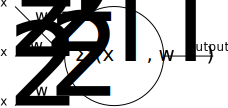
\includegraphics[width=0.5\textwidth]{out/perceptron.eps}
  \caption{Perceptron}
  \label{fig:perceptron}
\end{figure}
\FloatBarrier

\subsection{Multi Layer Perceptron}

\begin{itemize}
  \item Multi layer neural network where every perceptron in a layer is
        connected to every neuron in the adjacent layers
    \begin{itemize}
      \item A single input layer with as many neurons as they are input
            parameters
      \item Several inner layers
      \item A single output layer with as many neurons as they are outputs
    \end{itemize}
  \item Each layer represents a combination of features
    \begin{itemize}
      \item e.g. phonemes -> words -> sentences
    \end{itemize}
  \item A non linear multi layer perceptron with a single inner layer with
        enough neurons can learn any continuous function (universal
        approximation theory)
\end{itemize}

\begin{figure}[h!]
  \centering
  \includegraphics[width=0.5\textwidth]{out/multi_layer_perceptron.eps}
  \caption{Multi Layer Perceptron}
  \label{fig:multi_layer_perceptron}
\end{figure}
\FloatBarrier

\subsubsection{Learning Task}

\begin{itemize}
  \item Supervised learning given a set of inputs and the expected output
  \item Optimise the error function \ref{eq:mlp_e} to obtain the smallest value
        of $E$ by selecting new values of the weights $W$
  \item Computationally difficult to do using traditional optimisation methods
        (e.g. steepest-descent, Newton, etc.)
  \item Classic method for MLP is using backpropagation algorithm
    \begin{itemize}
      \item Two pass approach
      \item Calculate error of output layer
      \item Calculate weight updates of next layer back in turn
    \end{itemize}
\end{itemize}

\begin{align}
  E &= \frac{1}{n} \sum^{n}_{t=1} E(x')                   \\
    &= \frac{1}{n} \sum^{n}_{t=1} (F(x', W) - y_{t})^{2}
  \label{eq:mlp_e}
\end{align}

\subsection{Self Organised Maps}

\begin{itemize}
  \item a.k.a Kohonen neural network
  \item Unsupervised neural network
  \item Maps data from a high dimensionality to a 2D lattice
\end{itemize}

\begin{figure}[h!]
  \centering
  \includegraphics[width=0.8\textwidth]{out/som_training.eps}
  \caption{Self Organising Map Training}
  \label{fig:som_training}
\end{figure}
\FloatBarrier

Training:

\begin{enumerate}
  \item[1] A new input vector is selected
  \item[2] The node with a weight vector closest to the input vector (best
           matching unit) is found
  \item[3] The weight vector of the BMU and it's neighbours is modified to
           bring them closer to the input vector
\end{enumerate}

\subsection{Deep Learning}

\begin{itemize}
  \item A neural network with lots ($\geq 10$) inner layers
  \item More inner layers allows construction/recognition of higher level
        features
\end{itemize}

Types:

\begin{itemize}
  \item Purely supervised (deep NN)
    \begin{itemize}
      \item Trained using classic methods (e.g. backpropagation)
      \item Results in very slow training times due to network size
    \end{itemize}

  \item Semi-supervised (deep belief networks)
    \begin{itemize}
      \item Build inner layers incrementally in an unsupervised way
      \item Add a final supervised layer
    \end{itemize}

  \item Generative methods (convolutional NN)
    \begin{itemize}
      \item Each layer applies a "filter" to the data to reduce its
            dimensionality
      \item Commonly used with image/signal processing
    \end{itemize}
\end{itemize}

\subsubsection{Training semi-supervised networks}

\begin{enumerate}
  \item[1] Train first layer in an unsupervised manner
  \item[2] Fix first layer parameters and train second layer using the output of
           the first layer as unsupervised input to the second
  \item[3] Repeat for all inner layers
  \item[4] Use the outputs of the final layer as inputs to a supervised layer
           and train using the raining data outputs
  \item[5] Free all parameters and train entire network using a supervised
           approach using existing weights as initial values
\end{enumerate}

\subsubsection{Restricted Boltzmann machine}

\begin{itemize}
  \item Unsupervised neural network that learns a probability distribution over
        a set of inputs
  \item The result is it will learn to recognise recurrent patterns
\end{itemize}

\subsubsection{Convolutional Neural Network}

\begin{itemize}
  \item Each layer combines "patches" from the previous layer
  \item Compresses larger problems into smaller sets of features
  \item Filters are usually manually defined (i.e. not learned)
  \item Output of filtering is used to train a supervised model
  \item Requires neighbourhood regularity in input data (i.e. areas of a certain
        colour in an image)
\end{itemize}

\section{Memetic Algorithms}
\label{sec:ma}

\begin{itemize}
  \item Derived form the concept of traits spreading from person to person
  \item Combines conventional genetic algorithm (global search) with local
        search
  \item Global search allows exploration of entire problem space
  \item Local search allows exploration of neighbourhood of each individual to
        attempt to improve its fitness
\end{itemize}

\Para{Pseudocode}

\begin{listing}[h]
  \begin{minted}{python}
    population = init_random_population()
    iteration = 0
    while iteration < num_interations:
      evaluate(population)
      for i in range(len(population)):
        population[i] = select_local_best(population[i])
      population = selection(population)
      population = crossover(population)
      population = mutation(population)
      iteration++
    best = get_best_individual(population)
    return best
  \end{minted}
  \caption{Memetic algorithm pseudocode}
  \label{listing:ma_pseudocode}
\end{listing}

\subsection{Motivation}

\begin{itemize}
  \item When decomposing complex problems, subproblems may be easier to solve
        using either GA or local search
  \item Fast to reach optimal solution using domain specific knowledge in local
        search operator
  \item Domain knowledge in local search operator can "repair" bad individuals
        found by a GA
\end{itemize}

\subsection{Design considerations}

\Para{Baldwinism vs Lamarckism}

Two alternative theories for transfer of traits between individuals of a
population.

\begin{description}
  \item[Baldwinism] \hfill \\
    \begin{itemize}
      \item Traits acquired by an individual can be passed to its offspring
      \item e.g. replace an individual with its fitter neighbour
    \end{itemize}

  \item[Lamarckism] \hfill \\
    \begin{itemize}
      \item Traits acquired by an individual cannot be passed to its offspring
      \item e.g. individual inherits fitness but not genotype
    \end{itemize}

\end{description}

\Para{When to apply local search?}

\begin{itemize}
  \item After selection
  \item After crossover
  \item After mutation
\end{itemize}

\Para{In which stage of the genetic algorithm lifecycle?}

\begin{itemize}
  \item Uniformly throughout all iterations
  \item More in earlier or later iterations
\end{itemize}

\Para{Scope of local search?}

\begin{itemize}
  \item Entire population
  \item Probability of local search (fitness proportionate)
  \item Only individuals with specific range of fitness values
\end{itemize}

\Para{Choice of local search operator}

\begin{itemize}
  \item Use multiple, each of which having a fixed probability of being applied
  \item Have a fixed mapping of individuals to operator (domain specific)
  \item Evolve the operator choice using a GA
\end{itemize}

\Para{Other design issues}

\begin{itemize}
  \item Size of neighbourhood for local search
  \item Size of variations to make during local search operation
\end{itemize}

\Para{Diversity control}

\begin{itemize}
  \item Memetic algorithms naturally favour exploitation over exploration
  \item To ensure good evolution additional exploration must be done
  \item One option is to increase local search neighbourhood
\end{itemize}

\section{Swarm Intelligence}
\label{sec:swarm}

\begin{itemize}
  \item System of "items" collaborating to solve a task
  \item No external guidance/arbitration/synchronisation
\end{itemize}

\subsection{Ant Colony Optimisation}

\begin{itemize}
  \item Key concept is stigmergy, the indirect communication between individuals
        in the system through the environment
  \item In ants this is done though a pheromone trail deposited by ants as they
        explore a path
  \item Ants will always prefer to follow the path with the strongest pheromone
        trail
  \item Can be applied to any problem assuming it can be represented as a graph
    \begin{itemize}
      \item e.g. Ant-Miner: An unsupervised machine learning framework that
            constructs rules that identify patters in a set of input data.
    \end{itemize}
\end{itemize}

\subsubsection{Example: Travelling Salesperson Problem}

Close problem to actual ant colony movement.

\begin{itemize}
  \item Graph $G(N, E)$: $N$ are cities and $E$ are routed between cities
  \item $d_{i,j}$ is the fixed cost of travelling between cities $i$ and $j$
  \item Edge cost is given by a combination of:
    \begin{enumerate}
      \item[1] Static cost: $\eta(r, s) = \frac{1}{d_{r,s}}$
      \item[2] Dynamic trace: $\tau(r, s)$ deposited by ants (initially zero)
    \end{enumerate}
  \item All ants must visit all nodes in an iteration (a tour)
  \item At the end of an iteration all edges that are on the best tour receive
        additional pheromone
  \item At each iteration the pheromone count for all nodes may be reduced to
        reduce the chances of unpopular edges being selected in a tour
  \item Stopping criteria is either stagnation or a maximum number of iterations
    being performed.
\end{itemize}

\Para{Pseudocode}

\begin{listing}[h]
  \begin{minted}{python}
    graph = init_graph(d)
    place_ants()
    while not stopping_criteria:
      while not all_cities_visited:
        for a in ants:
          move_to_next_city(a)
      place_ants()
      graph = update_graph(tau)
    return graph
  \end{minted}
  \caption{Ant colony optimisation for TSP pseudocode}
  \label{listing:aco_for_tsp_pseudocode}
\end{listing}
\FloatBarrier

\subsection{Particle Swarm Optimisation}

\begin{itemize}
  \item General purpose optimisation for continuous variables
  \item Each particle searches for the optimum
  \item Each particle is moving with a velocity
  \item Each particle knows its last position and the position of its best
        result so far
  \item A particle has a neighbourhood associated with it
  \item A particle knows the position of the most optimal particle in its
        neighbourhood
\end{itemize}

\subsubsection{Neighbourhood types}

\begin{figure}[h!]
  \centering
  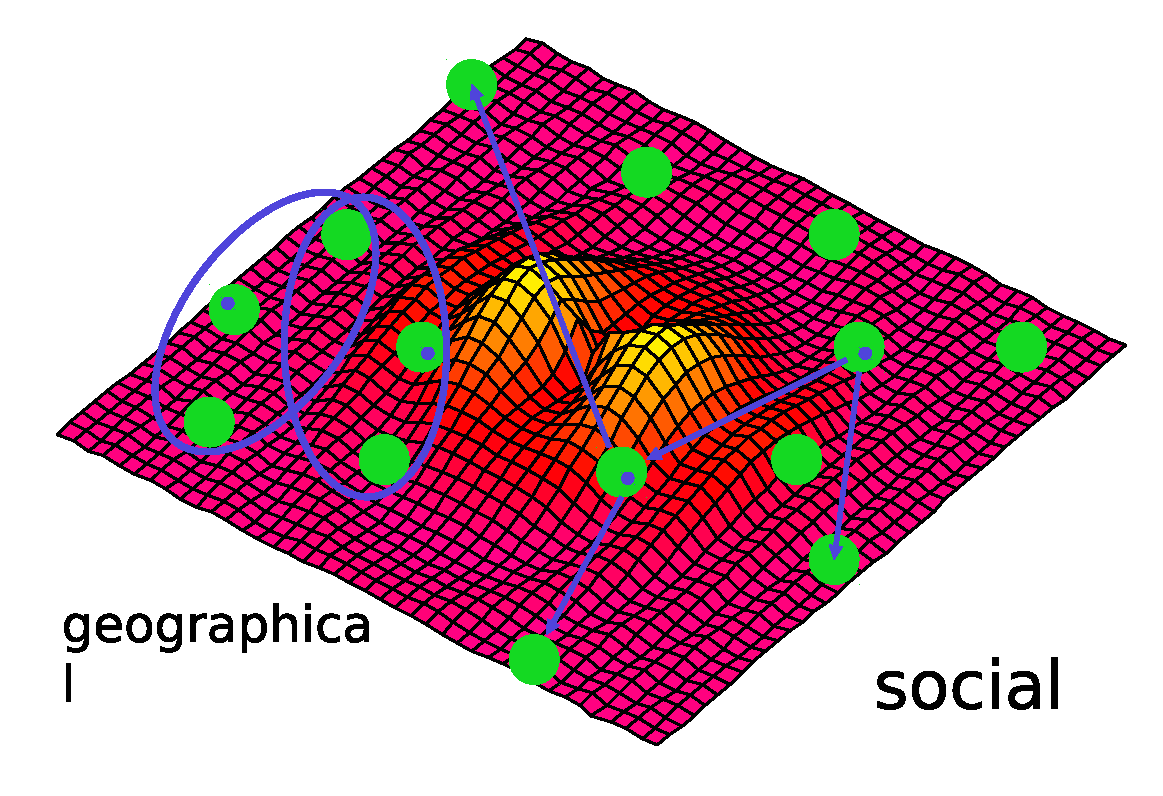
\includegraphics[width=0.6\textwidth]{graphics/pso_neighbourhoods_1.eps}
  \caption{Geographical and social neighbourhoods}
  \label{fig:pso_neighbourhoods_1}
\end{figure}
\FloatBarrier

\begin{figure}[h!]
  \centering
  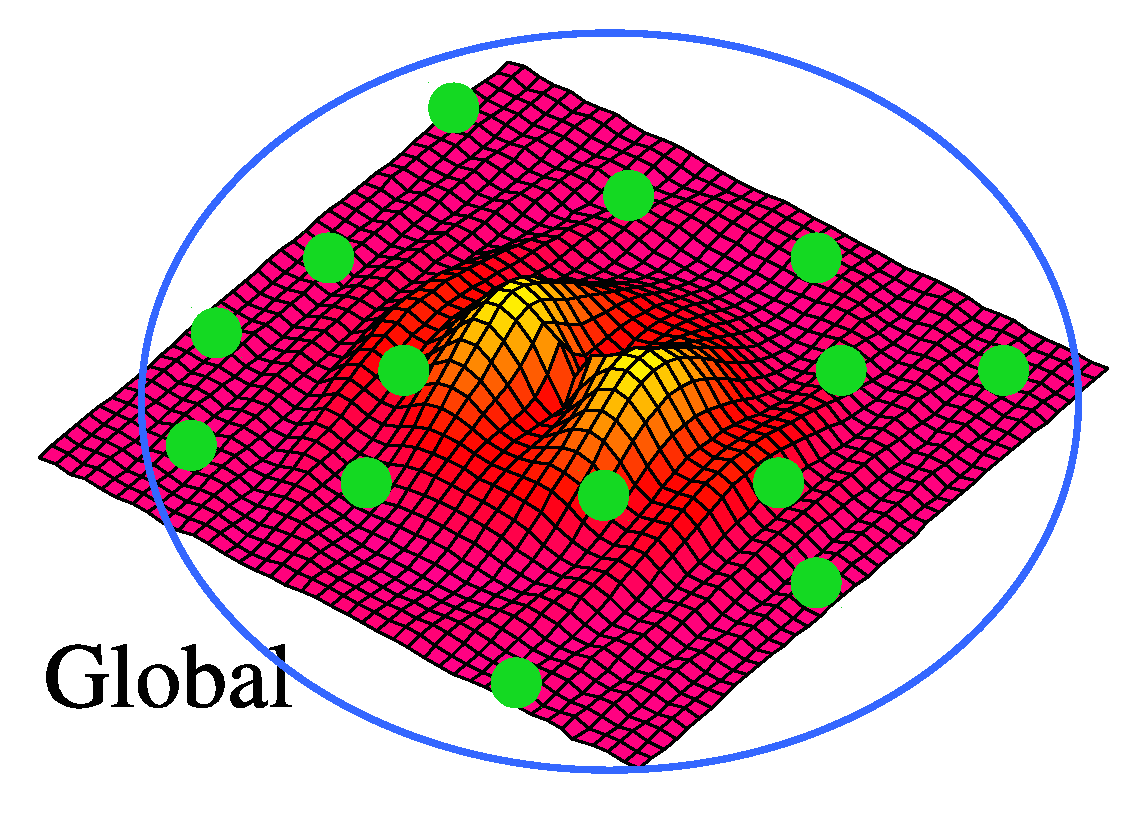
\includegraphics[width=0.6\textwidth]{graphics/pso_neighbourhoods_2.eps}
  \caption{Global neighbourhood}
  \label{fig:pso_neighbourhoods_2}
\end{figure}
\FloatBarrier

\begin{figure}[h!]
  \centering
  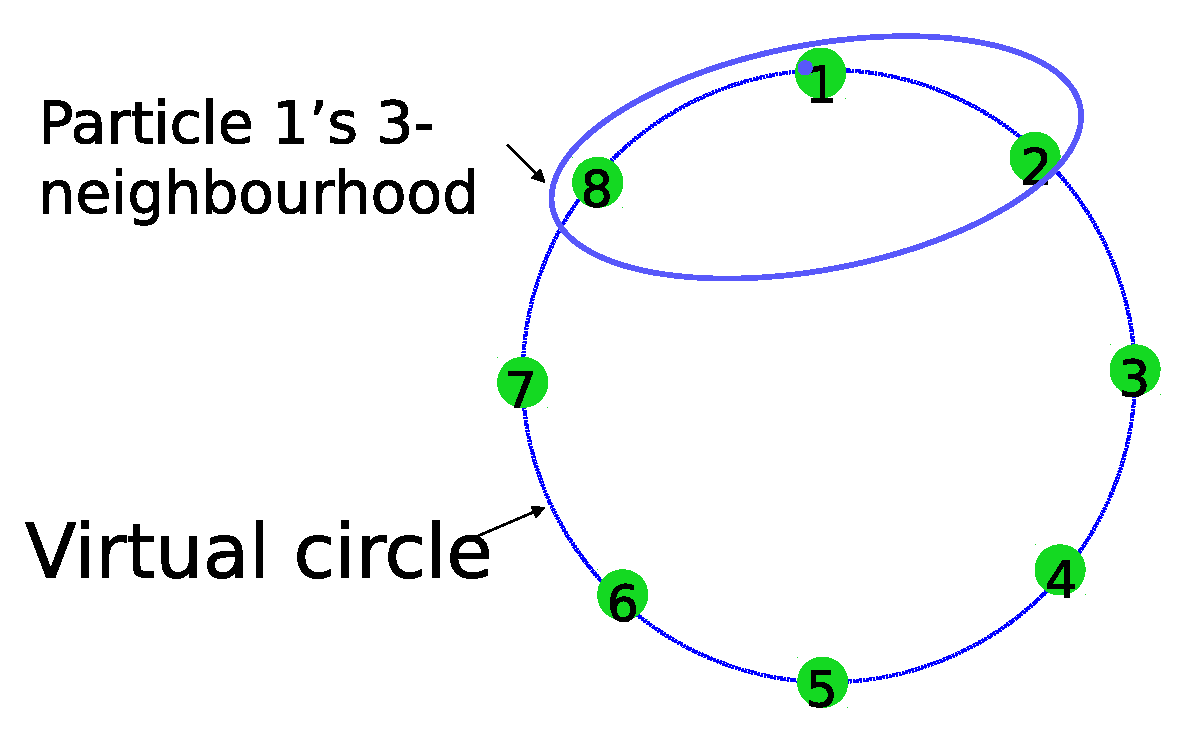
\includegraphics[width=0.6\textwidth]{graphics/pso_neighbourhoods_3.eps}
  \caption{Circular neighbourhood}
  \label{fig:pso_neighbourhoods_3}
\end{figure}
\FloatBarrier

\subsubsection{Algorithm}

\begin{itemize}
  \item In each time step a particles velocity and position are updated as per
        equations \ref{eq:particle_vel_update} and \ref{eq:particle_pos_update}
  \item Particle velocity is limited to a fixed $max\_velocity$
\end{itemize}

\begin{equation}
  \label{eq:particle_vel_update}
  \begin{split}
    velocity = \: &a * velocity \: + \\
                  &b * (neighbourhood\_best - position) + \\
                  &c * (local\_best - position) \\
    velocity = \: &max(velcoity, max\_velocity)
  \end{split}
\end{equation}

\begin{equation}
  \label{eq:particle_pos_update}
  position = position + velocity
\end{equation}

\Para{Pseudocode}

\begin{listing}[h]
  \begin{minted}{python}
    particles = random_initial_particles()

    while not stopping_criteria:
      for p in particles:
        fitness = evaluate(p)

        if fitness > p.best:
          p.best = fitness
        if fitness > global_best:
          global_best = fitness

      for p in particles:
        update_velocity(p)
        update_position(p)
  \end{minted}
  \caption{Particle swarm optimisation pseudocode}
  \label{listing:pso_pseudocode}
\end{listing}
\FloatBarrier

\section{Cellular Automata}
\label{sec:ca}

\begin{itemize}
  \item Biological inspiration is cells and cell reproduction
  \item Idea of a self replicating system
  \item Discrete systems that model complex behaviour using simple logical rules
  \item Collection of cells
    \begin{itemize}
      \item Oriented in an $n$-dimensional grid
      \item Have a state (taken from a finite set)
      \item Have a neighbourhood
      \item State of cell in next time step is computed using rules
      \item Rules define states based on current state of cells in
            neighbourhood
    \end{itemize}
  \item A cellular automation is evaluated generation by generation until some
        stopping criteria are reached or it is stopped manually
\end{itemize}

\subsection{1D eight rule CA}

\begin{itemize}
  \item 1 dimensional gird
  \item Two states: 1 or 0
  \item 8 rules
  \item 256 possible rule sets
\end{itemize}

Classification of behaviour for different rule sets:

\begin{description}
  \item[Class 1: Uniformity] \hfill \\
    Rapidly converge to a uniform state
  \item[Class 2: Repetition] \hfill \\
    Rapidly converge to a repetitive stable state
  \item[Class 3: Random] \hfill \\
    Appear to remain in a random state
  \item[Class 4: Complexity] \hfill \\
    Form areas of repetitive or stable sates while also forming structures which
    interact with each other in complex ways
\end{description}

\subsection{2D cellular automata}

\begin{itemize}
  \item Very similar to 1 dimensional CA but with larger neighbourhood
  \item Larger neighbourhood means more complex rules (due to larger number of
        possible neighbourhood states for a given cell)
  \item Rule set may become too large to explicitly define
\end{itemize}

\subsubsection{Neighbourhoods}

\begin{figure}[h!]
  \centering
  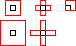
\includegraphics[width=0.5\textwidth]{out/2d_ca_neighbourhoods.eps}
  \caption{Examples of neighbourhoods}
  \label{fig:2d_ca_neighbourhoods}
\end{figure}
\FloatBarrier

Left to right, top to bottom:

\begin{itemize}
  \item Moore
  \item Von Neumann
  \item Margolus
  \item Extended Moore
  \item Extended Von Neumann
\end{itemize}

When a neighbourhood is at the edge of the 2D matrix it can either be cropped to
form a smaller neighbourhood or wrapped around the matrix.

\subsection{The Game Of Life}

\Para{Goals}

A "lifelike" result with a simple set of rules.

\begin{enumerate}
  \item[1] There should be no initial patters that can be proved to allow a
           population to grow indefinitely
  \item[2] There should be initial patters that appear to grow without limit
  \item[3] There should be initial patters that grow/change before coming to an
           end in one of three ways:
    \begin{itemize}
      \item Fading away completely (overcrowding or too sparse)
      \item Settling into a stable state that does not change between
            generations
      \item Entering an oscillating state
    \end{itemize}
\end{enumerate}

\Para{Rules}

Whether a cell is on or off (lives or dies) in the next iteration is determined
by the following rules:

\begin{description}
  \item[Loneliness] \hfill \\
    A live cell with fewer then two live neighbours dies.
  \item[Companionship] \hfill \\
    A live cell with two or three live neighbours lives.
  \item[Overcrowding] \hfill \\
    A live cell with more then three live neighbours dies.
  \item[Reproduction] \hfill \\
    A dead cell with exactly three live neighbours becomes live.
\end{description}

\Para{Constructs}

Groups of cells that exhibit specific behaviour.

\begin{description}
  \item[Still life] \hfill \\
    Constructs that have reached a state that will not change between
    generations without interaction from other constructs.
  \item[Oscillating constructs] \hfill \\
    Constructs that cycle between two or more states over a given number of
    generations.
  \item[Moving constructs] \hfill \\
    Constructs that move across the grid over time, usually by means of an
    oscillating set of states.
\end{description}

\Para{Computation}

Can perform simple computations using glider guns to create "sliding block
memory" from which logic gates can be simulated.

Can create state machines (using sliding block memory as a counter) to form a
universal Turing machine.

\subsubsection{Variants}

\begin{description}
  \item[3D cellular automata] \hfill \\
    Same principal as 1D and 2D but with a larger neighborhood.

  \item[Different cell shapes] \hfill \\
    Assuming a shape can be oriented on a grid (tessellated) and assigned a
    neighbourhood then it can be used in a cellular automation.

    e.g. Triangles and hexagons have been used.

  \item[Probabilistic rules] \hfill \\
    Have a set of rules that have probability weightings instead of being purely
    deterministic.

  \item[Continuous cellular automata] \hfill \\
    Using continuous values rather than discreet states.

  \item[Nested cellular automata] \hfill \\
    Used to simulate a hierarchical system.

    e.g. County $\rightarrow$ City $\rightarrow$ Person $\rightarrow$ Cell

\end{description}

\subsubsection{Applications}

\begin{description}
  \item[Computer graphics] \hfill \\
    Performing filter computations to an image.

    e.g. Blurring is an operation that modifies each pixel depending on the
    states of the pixels in its neighbourhood.

  \item[Game development] \hfill \\
    Used for world generation, given a random seed (states in initial
    generation).

  \item[Cryptography] \hfill \\
    One way function used for public key encryption.

    Given a rule set it is easy to calculate future states given an early
    generation, but very difficult to calculate past states given a later
    generation.

  \item[Simulation] \hfill \\
    Various biological and physical simulations.

    e.g. Pattern formation, cell development, fluid flow, etc.

  \item[Fractals] \hfill \\
    Generation of patterns based on simple self replication rules.

\end{description}

\section{Membrane Computing}
\label{sec:membrane}

TODO

\section{DNA Computing}
\label{sec:dna}

Performing computations on biological devices, specifically DNA.

\subsection{Structure of DNA}

\begin{itemize}
  \item Asymmetric double helix
  \item Complimentary strands A-T and C-G
  \item $5^{\prime}$ denotes the front of a motif (upstream)
  \item $3^{\prime}$ denotes the end of a motif (downstream)
\end{itemize}

\subsection{Features useful for computation}

\begin{itemize}
  \item Massive parallelism
    \begin{itemize}
      \item Small amount of DNA contains many strands
      \item When strings are randomised then a small volume of DNA will contain
            a large number of unique strings
    \end{itemize}

  \item Complementarity
    \begin{itemize}
      \item Know that if a string binds to a larger string then the larger
            string must contain the complementarity string to the smaller string
      \item e.g. if $5^{\prime}$ ACGT $3^{\prime}$ binds to a longer string
            $S$, you know that $S$ contains the string $3^{\prime}$ TGCA
            $5^{\prime}$
    \end{itemize}
\end{itemize}

\subsection{Experimental Techniques}

\subsubsection{Polymerase Chain Reaction}

Used to replicate DNA, creating many copies of the base pairs.

\begin{enumerate}
  \item[1] Separate two base strands at low heat
  \item[2] Add base pairs, primer sequences and DNA polymerise
    \begin{itemize}
      \item Creates double stranded DNA from single strand
      \item Primer sequence creates seed from which the double stranded DNA
            grows
    \end{itemize}
  \item[3] Repeat, DNA grows exponentially
\end{enumerate}

\subsubsection{Electrophoresis}

\begin{itemize}
  \item Phosphate backbone of DNA is negatively charged
  \item Migration of DNA to agaraose gel shows visible pores on the gel surface
  \item An electric field is placed over the DNA to force migration
  \item Size of DNA fragments is determined by pore size
\end{itemize}

\subsection{Solving the Hamiltonian Path Problem}

Given a directed graph $G=(V,E)$, $V_{start}$ and $V_{end}$, is there a directed
path starting at $V_{start}$ and finishing at $V_{end}$ that visits all vertices
exactly once.

\subsubsection{Non-deterministic approach}

\begin{enumerate}
  \item[1] Generate many random paths through $G$
  \item[2] Keep only paths that start at $V_{start}$ and end at $V_{end}$
  \item[3] Keep only paths with length $n = |V|$
  \item[4] Keep only paths that visit each vertex once
  \item[5] If any paths remain then result is true, if no paths remain result is
           false
\end{enumerate}

Exploits:

\begin{description}
  \item[Massive parallelism] to take care of non-deterministic nature of
                             algorithm
  \item[Complementarity] is used to select and filter solutions
\end{description}

\subsubsection{Stage 1: Initialisation}

\Para{Vertex and edge encoding}

\begin{itemize}
  \item A vertex is encoded by a 20-mer length string
  \item An edge is encoded by the back 10-mer and the front 10-mer from the two
        connected vertices
  \item Edges for $V_{0}$ ($V_{start}$) and $V_{n}$ ($V_{end}$) contain the full
        string for the start and end vertices (i.e. so are 30-mer or 40-mer)
\end{itemize}

\Para{Building random paths}

50 picomol of the complimentary sequence ($v^{\prime}$) (except $V_{0}$ and
$V_{n}$) is mixed with 50 picomol of each edge encoding

\subsubsection{Stage 2: PCR amplification}

\begin{itemize}
  \item Implements step 2
  \item Amplify using primers: $V_{0}$ and $V^{\prime}_{n}$
  \item PCR will replicate everything with $V_{0}$ and $V_{n}$ at the ends
\end{itemize}

\subsubsection{Stage 3: Selecting paths of length $|V|$}

\begin{itemize}
  \item Double stranded DNA that represents paths going through exactly $n$
        vertices are selected
  \item Based on size measured through electrophoresis
\end{itemize}

\subsubsection{Stage 4: Selecting paths that visit all vertices}

\begin{itemize}
  \item Double strands from stage 3 are denatured
  \item Put into a mix with $V^{\prime}_{1}$ which are magnetically attached to
        beads
  \item Strands containing $V_{1}$ anneal to $V^{\prime}_{1}$
  \item Strands not containing $V_{1}$ are washed away
  \item Repeat for all vertices (except $V_{0}$ and $V_{n}$)
\end{itemize}

\subsubsection{Stage 5: Result}

\begin{itemize}
  \item Remaining strands after stage 4 undergo PCR and electrophoresis
  \item If any strands remain in the gel then $G$ has a Hamiltonian path
\end{itemize}

\subsection{DNA origami}

\begin{itemize}
  \item Forcing DNA to form complex shapes and structures by giving it a certain
        sequence
  \item Structures formed of:
    \begin{description}
      \item[Scaffold] \hfill \\
        A long single stranded DNA string
      \item[Staples] \hfill \\
        A set of short unique strings that bind to the scaffold in specific
        places
    \end{description}
  \item Designed using the De Brujin sequence
\end{itemize}

\end{document}
